\documentclass[letterpaper]{article}
\usepackage[margin=1in]{geometry}
\usepackage[utf8]{inputenc}
\usepackage{textcomp}
\usepackage{amssymb}
\usepackage{natbib}
\usepackage{graphicx}
\usepackage{gensymb}
\usepackage{amsthm, amsmath, mathtools}
\usepackage[dvipsnames]{xcolor}
\usepackage{enumerate}
\usepackage{mdframed}
\usepackage[most]{tcolorbox}
\usepackage{csquotes}
% https://tex.stackexchange.com/questions/13506/how-to-continue-the-framed-text-box-on-multiple-pages

\tcbuselibrary{theorems}

\newcommand{\R}{\mathbb{R}}
\newcommand{\Z}{\mathbb{Z}}
\newcommand{\N}{\mathbb{N}}
\newcommand{\Q}{\mathbb{Q}}
\newcommand{\C}{\mathbb{C}}
\newcommand{\code}[1]{\texttt{#1}}
\newcommand{\mdiamond}{$\diamondsuit$}
\newcommand{\PowerSet}{\mathcal{P}}
\newcommand{\Mod}[1]{\ (\mathrm{mod}\ #1)}
\DeclareMathOperator{\lcm}{lcm}

%\newtheorem*{theorem}{Theorem}
%\newtheorem*{definition}{Definition}
%\newtheorem*{corollary}{Corollary}
%\newtheorem*{lemma}{Lemma}
\newtheorem*{proposition}{Proposition}


\newtcbtheorem[number within=section]{theorem}{Theorem}
{colback=green!5,colframe=green!35!black,fonttitle=\bfseries}{th}

\newtcbtheorem[number within=section]{definition}{Definition}
{colback=blue!5,colframe=blue!35!black,fonttitle=\bfseries}{def}

\newtcbtheorem[number within=section]{corollary}{Corollary}
{colback=yellow!5,colframe=yellow!35!black,fonttitle=\bfseries}{cor}

\newtcbtheorem[number within=section]{lemma}{Lemma}
{colback=red!5,colframe=red!35!black,fonttitle=\bfseries}{lem}

\newtcbtheorem[number within=section]{example}{Example}
{colback=white!5,colframe=white!35!black,fonttitle=\bfseries}{def}

\newtcbtheorem[number within=section]{note}{Important Note}{
        enhanced,
        sharp corners,
        attach boxed title to top left={
            xshift=-1mm,
            yshift=-5mm,
            yshifttext=-1mm
        },
        top=1.5em,
        colback=white,
        colframe=black,
        fonttitle=\bfseries,
        boxed title style={
            sharp corners,
            size=small,
            colback=red!75!black,
            colframe=red!75!black,
        } 
    }{impnote}
\usepackage[utf8]{inputenc}
\usepackage[english]{babel}
\usepackage{fancyhdr}
\usepackage[hidelinks]{hyperref}

\pagestyle{fancy}
\fancyhf{}
\rhead{CSE 131}
\chead{Friday, May 12, 2023}
\lhead{Lecture 18}
\rfoot{\thepage}

\setlength{\parindent}{0pt}

\begin{document}

\section{Garbage Collection}
Now that we're working with memory in the heap, let's suppose we \emph{don't} have a lot of memory to work with. In this case, we need to think about \emph{garbage collection} as a way to get rid of unused memory so we can allocate memory for useful things. 

\subsection{Motivation}
Let's take a look at two examples to get an idea of what we're working with. 

\subsubsection{Motivation 1: Basic Garbage}
Recall the following code from class: 
\begin{verbatim}
(let (x (pair 1 2))
    (let (y (let (tmp (pair 10 20)) (+ (fst tmp) (snd tmp))))
        (let (p0 (+ (fst x) y))
            (let (p1 (+ (snd x) y))
                (pair p0 p1)
            )
        )
    )
)\end{verbatim}

After creating the final pair, the memory diagram looks like\footnote{For the sake of conciseness, we're showing the numbers without their tagged representation.}\footnote{Also, the \code{tmp} to \code{y} arrow indicates that we're \emph{reusing} that space.} 
\begin{center}
    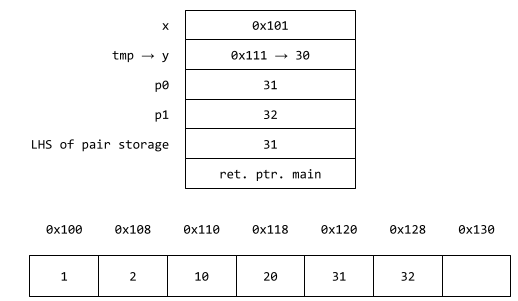
\includegraphics[scale=0.6]{../assets/stackHeapPairGC1.png}
\end{center}
Here, the stack is the top diagram while the heap is the bottom diagram. Note that \code{rax}\footnote{Which is storing the answer to our program} is \code{0x121}, and \code{r15}\footnote{Recall that \code{r15} will always point to the next available word in the heap} is \code{0x130}. 

\bigskip 

\textbf{Now, let's suppose} our heap only has five available words. \code{rax} will hold the result of \code{(+ (snd x) y)} (i.e., result of addition, which is a number). Immediately, we should notice that 
\begin{itemize}
    \item We don't have enough memory to allocate for the final pair!
    \item More importantly, however, the values in the heap at location \code{0x110} and \code{0x118} are \textbf{garbage}. Nothing in the stack (or a register) is referring to these values!  
\end{itemize}
To clarify, the idea is that any memory that is not reachable from the stack (or any registers) is considered garbage and can be reused. So, our goal is to get rid of the garbage so we have enough memory to allocate for the final pair. With this said, a high-level implementation of a basic garbage collector would look something like this. 
\begin{center}
    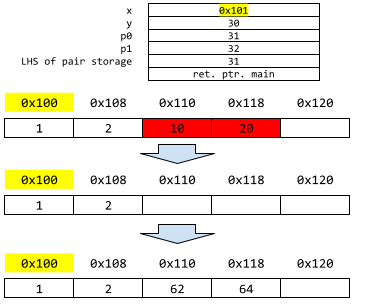
\includegraphics[scale=0.7]{../assets/stackHeapPairGCFix1.png}
\end{center}
So here's what's going on:
\begin{itemize}
    \item We've determined that the stuff at \code{0x110} and \code{0x118} are garbage, so we can get rid of them. 
    \item After that, we can \emph{compact the heap}, essentially moving \code{r15} back to \code{0x110}. After that, we can allocate memory for our next pair. 
    \item This gives us the desired result, with \code{rax} being \code{0x110}. 
\end{itemize}
A key observation here is that we didn't need to ``fix'' any memory addresses stored in the stack or in the heap itself. 

\subsubsection{Motivation 2: Slightly Complicated Garbage}
Consider the following code: 
\begin{verbatim}
    (fun (inc lst)
        (if (= lst nil)
            nil 
            (pair (+ (fst lst) 1) (inc (snd lst)))
        )
    )

    (inc (inc (pair 70 (pair 800 nil))))\end{verbatim}

After the second call to \code{inc} (i.e., after the first call to \code{inc} finishes), we have the following rough diagram:
\begin{center}
    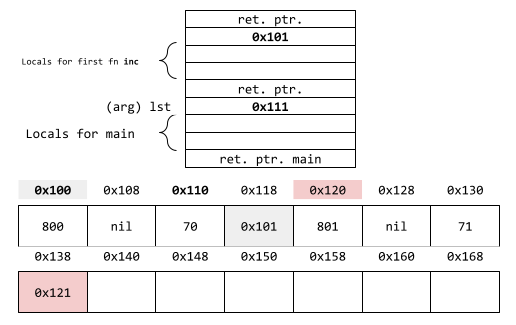
\includegraphics[scale=0.7]{../assets/stackHeapPairGC2.png}
\end{center}
The register \code{rax} would have value \code{0x131}. What is considered garbage? The first four words -- \code{0x100} through \code{0x118} -- are considered \textbf{garbage} since there's no references to those words anywhere in the stack. However, why is this the case?  
\begin{itemize}
    \item We'll define the stack as everything at an address higher than \code{rsp} to the top of \code{our\_code\_starts\_here}, but not anything lower address or above that. Therefore, we don't need to consider the following in the stack when deciding what is garbage: 
    \begin{center}
        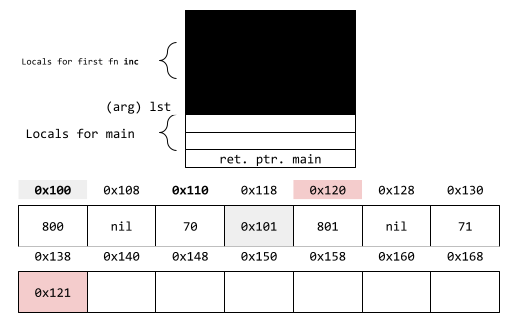
\includegraphics[scale=0.5]{../assets/stackHeapPairGC3.png}
    \end{center}

    \item So, as long as no references to \code{0x111} is in main, we can prove that it's garbage.
\end{itemize}
\textbf{Now, let's suppose} our heap only has eight available words. In this example, \code{rax} is \code{0x131}. As one might have suspected, we don't have any memory left to allocate the remaining pairs needed for this program; in particular, after we call the \code{inc} function with the pair that we got from our initial call to \code{inc}, we don't have enough memory to allocate another pair needed for the recursive call. So, we need to collect some garbage. Here's how we might go about this. 
\begin{center}
    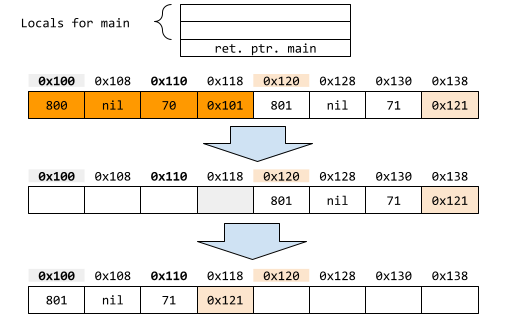
\includegraphics[scale=0.7]{../assets/stackHeapPairGCFix4.png}
\end{center}
So, here's what's going on: 
\begin{itemize}
    \item We determined that the first four words are garbage, since no items in the stack or any registers are referring to those four words in the heap. 
    \item We can compact the heap by moving \code{r15} to the beginning of our heap, thus allowing us to reuse the four words that are garbage. 
    \item Now that we have room in the heap, we can allocate the final pair and change \code{rax} to point to our final result.
\end{itemize}
Well, \emph{not quite}. Unlike the previous example, notice how we have a memory address in the heap that's referring to a memory address that's now garbage. That memory address has been relocated, so \textbf{we need to fix this.} Specifically, we need to change the value at \code{0x118} to point to \code{0x100}, not the garbage value at \code{0x120}! Likewise, any call to the stack that uses any memory addresses to the heap might need to be fixed before we can continue. 

\bigskip 

Therefore, we need to not only compact the heap, but also \emph{relocate/forward} all existing references.

\end{document}